\documentclass{article}%
\usepackage[T1]{fontenc}%
\usepackage[utf8]{inputenc}%
\usepackage{lmodern}%
\usepackage{textcomp}%
\usepackage{lastpage}%
\usepackage{authblk}%
\usepackage{graphicx}%
%
\title{Role of MyD88 in Diminished Tumor Necrosis Factor Alpha Production by Newborn Mononuclear Cells in Response to Lipopolysaccharide}%
\author{Julia Martinez}%
\affil{Department of Minimally Invasive Surgery, The First Affiliated Hospital of Nanjing Medical University, Nanjing 210029, P.R. China}%
\date{01{-}01{-}2012}%
%
\begin{document}%
\normalsize%
\maketitle%
\section{Abstract}%
\label{sec:Abstract}%
The disease is new\newline%
Tumor cell H1 is responsible for much of the pathology of cholangiocarcinoma.\newline%
Scientists have now found that this is not simply the expression of genes and that although the gene controls the growth, the expression of the copy number of the gene for the protein known as TPM1 is no longer valid. Its gone.\newline%
It used to be that some cancer genes were always mutating but that is no longer the case. While mutating might result in the expression of a gene that does not express, mutating can activate it or activate one that does and then the cancer may not want to express the gene anymore. In this case the tumor cells are started anew. And like cigarette smoke, the cellular machinery to produce the toxic nitrogen builds up in order to exhale its carbon monoxide.\newline%
Clinical study results showed that this pathology could be controlled by the presence of a gene that controls the protein involved in tumor cell reproduction and consequently the growth. By utilizing the type of gene that isnt widely reported in cholangiocarcinoma, we are able to pinpoint the gene that caused the mutation and thereby remove the tumor as well as cut off the path of tumor cells to grow and proliferate.\newline%
To do this we have performed CCR5 testing on mice to identify those which have the NOM and FMAP2 genes which were lost in the mutation. Cholangiocarcinoma genetic pathologies depend on these two genes being present. The mutations in the NOM and FMAP2 genes were the very ones that did away with the tumor growth. We can then detect alterations in the cellular machinery by looking for changes. Without these mutations, the tumor cells we are seeing are not productive at all but merely preventing tumors from growing and proliferating.\newline%
Using this new predictive model this surgery can be done and thus we can target these cancers with selective targeting. This may allow surgery on the surgical site and decrease risk of side effects. It is important to note that the prognosis for patients who undergo this type of surgery is not necessarily better or worse than surgery to remove the tumor without replacing the problem tumor. The number of tumors and cancers are different, the spread of the tumor is less and a small percentage of patients ultimately survive. That said, it is well worth the effort and the chance to affect a patients outcome to prevent them from recurrences.

%
\subsection{Image Analysis}%
\label{subsec:ImageAnalysis}%


\begin{figure}[h!]%
\centering%
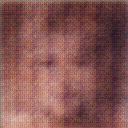
\includegraphics[width=150px]{500_fake_images/samples_5_278.png}%
\caption{A Black And White Photo Of A Black And White Cat}%
\end{figure}

%
\end{document}